\section{Outer Optimisation Routine}
The unconstrained outer optimisation over the scalar value $R \in \R^+$, the radius of our domain $B_R(\vec{0})$, is carried out using \href{https://github.com/JuliaNLSolvers/Optim.jl}{Optim.jl}'s implementation \parencite{2023-optim-jl} of the \gls{lbfgs} optimisation method \parencite{1989-lbfgs}, an extension of BFGS for low-memory usage, using an estimate for the gradient based on \gls{ad} techniques.

As part of a comparison between multiple optimisation approaches, \gls{lbfgs} outperformed the Nelder-Mead and Newton trust region methods for our case, converging extremely quickly within only 3 iterations, 10 function calls and 10 evaluations of the gradient.
While the downhill simplex method by \citeauthor{1965-nelder-mead} did not converge to the desired local minimum (cf. \Cref{fig:outer-optimisation}), the trust region method using Newton's method to solve a quadratic model for each subproblem \parencite{1982-trust-region} also converged in only 3 iterations with only 4 function, gradient and Hessian evaluations.
Again, the values of the gradient and Hessian (in the case of a one-dimensional optimisation, simply the first and second derivatives), are obtained using \glstext{ad}.

The \gls{lbfgs} method converged with $\norm{\nabla E(R)} \approx 10^{-11}$ while the Newton trust region method converged at $\norm{\nabla E(R)} \approx 10^{-9}$.
The entire optimisation routine with \gls{lbfgs}, including function and gradient evaluations (solving a $12 \times 12$ linear system), takes \SI{28 \pm 4}{\milli\second} on an Intel\textregistered \, i7-5600U CPU running at \SI{2.6}{\giga\hertz}.

\begin{figure}[H]
  \centering
  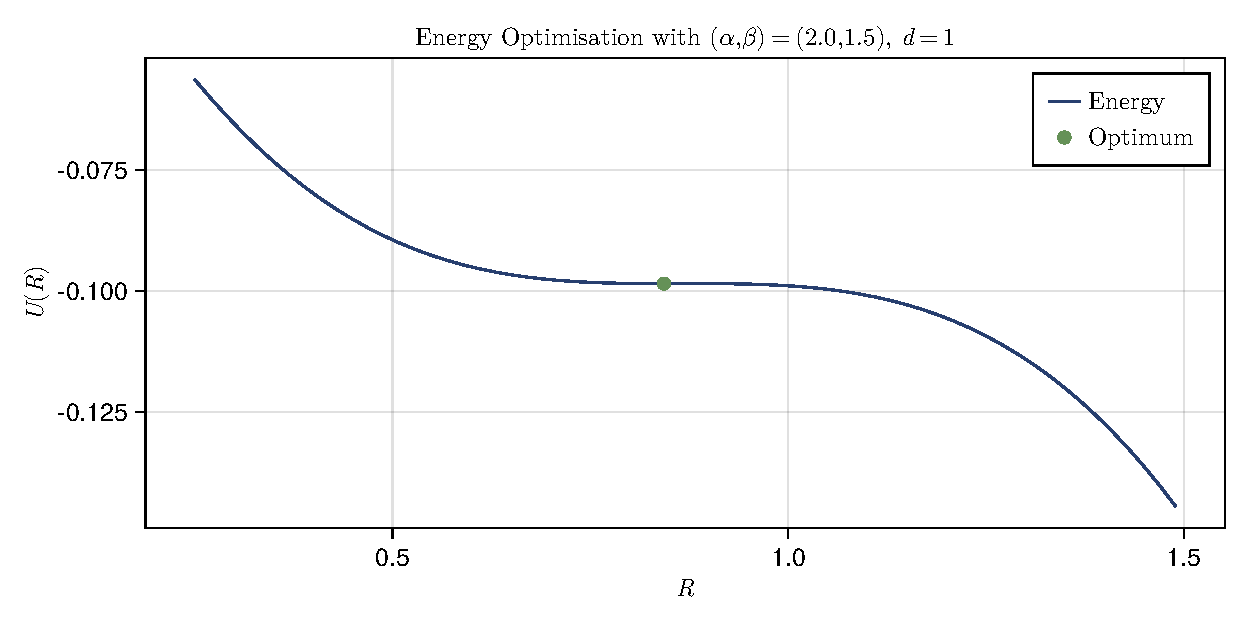
\includegraphics[width=0.8\linewidth]{results/known-analytic/outer-optimisation.pdf}
  \caption[Outer Optimisation Routine]{The total potential $U$ as a function of the support radius $R$. This is the goal function minimised by the outer optimisation routine.}
  \label{fig:outer-optimisation}
\end{figure}

Note that using this setup, the operators themselves do not need to be recomputed upon a change in $R$, cf. \Cref{eq:full-attrep-operator}.
The provided implementation uses \gls{lru} caching to automatically store operators for a given parameter set and order $N$.

\begin{lemma}{Unique Energy Minimum}{attrep-energy-min}
  Assuming an $N=1$ expansion of the density distribution $\rho$ according to \Cref{eq:ansatz} with $m \in \N_0$, for an attractive-repulsive interaction potential $K_{\alpha, \beta}(r) = \frac{r^\alpha}{\alpha} - \frac{r^\beta}{\beta}$, the energy minimum $E_{\rm min} = E(R_{\rm min})$ is unique and given by
  $$R_{\rm min} = \left(\sfrac{\bar{I}_{m,0}^{\alpha,\beta}}{\bar{I}_{m,0}^{\alpha,\alpha}}\right)^\frac{1}{\alpha-\beta}\,,$$
  with $\bar{I}_{m,n}^{\alpha,\alpha}$ as given in \Cref{eq:0th-coeff-of-I}.
\end{lemma}
\begin{proof}
  Starting from the total energy given in \Cref{eq:total-energy-for-ansatz}, we obtain the first derivative as
  $$\frac{\partial E}{\partial R} = 1$$

  Because $\alpha > \beta$, we have $\lim_{r \goesto \infty} K_{\alpha,\beta}(r) = \infty$ and more importantly,
  $$\lim_{R \goesto \infty} E(R) = \lim_{R \goesto \infty} \frac{R^{2d+\alpha}}{\alpha} U^{(\alpha)} - \frac{R^{2d+\beta}}{\beta} U^{(\beta)} = \infty\,,$$
  when both $U^{(\alpha)}, U^{(\beta)} < \infty$, telling us that $R_{\rm min}$ must be a minimum!
\end{proof}

There is strong numerical evidence that the energy minimum is also unique for $N > 1$.
Despite significant effort, this remains difficult to prove.
Even for $N = 2$, attempting a direct substitution of $\vec{\rho}$ through the explicit inversion of a $2 \times 2$ matrix, leads to finding the roots of a quintic polynomial for which it is well-known that no explicit formula exists.
